\documentclass{article}
% translate with >> pdflatex -shell-escape <file>

% This file is an extract of the PGFPLOTS manual, copyright by Christian Feuersaenger.
% 
% Feel free to use it as long as you cite the pgfplots manual properly.
%
% See
%   http://pgfplots.sourceforge.net/pgfplots.pdf
% for the complete manual.
%
% Any required input files (for <plot table> or <plot file> or the table package) can be downloaded
% at
% http://www.ctan.org/tex-archive/graphics/pgf/contrib/pgfplots/doc/latex/
% and
% http://www.ctan.org/tex-archive/graphics/pgf/contrib/pgfplots/doc/latex/plotdata/

\usepackage{pgfplots}
\pgfplotsset{compat=newest}

\pagestyle{empty}

\begin{document}
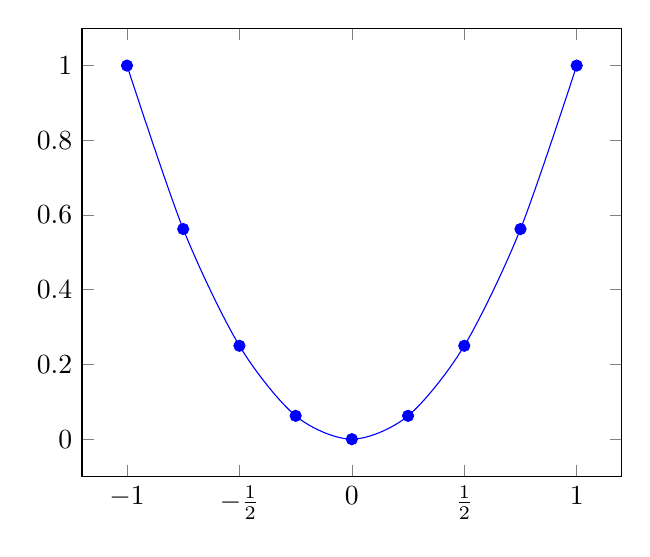
\begin{tikzpicture}
\begin{axis}[
	xtick={-1.5,-1,...,1.5},
	xticklabels={%
		$-1\frac 12$,
		$-1$,
		$-\frac 12$,
		$0$,
		$\frac 12$,
		$1$},
	% note: \frac can be done automatically:
	% xticklabel style={/pgf/number format/frac},
]
\addplot[smooth,blue,mark=*] 
coordinates {
	(-1,    1)
	(-0.75, 0.5625)
	(-0.5,  0.25)
	(-0.25, 0.0625)
	(0,     0)
	(0.25,  0.0625)
	(0.5,   0.25)
	(0.75,  0.5625)
	(1,     1)
};
\end{axis}
\end{tikzpicture}
\end{document}
